\chapter{Generative Deep Learning}\label{chp:generative_deep_learning}

\section{Intro to Deep Generative Models}


What Is Generative Modeling?

Generative modeling can be broadly defined as follows:
Generative modeling is a branch of machine learning that involves training a model to produce new data that is similar to a given dataset~\cite{foster2022generative}.

Discriminative models vs Generative models

\paragraph{The Generative Modeling Framework}

\begin{itemize}
	\item We have a dataset of Observations $\mathbf{X}$.
	\item We assume that the observations have been generated according to some unknown distribution \(\mathcal{P}_{\textrm{data}}\)
	\item We want to build a generative model \(\mathcal{P}_{\textrm{model}}\) that mimics \(\mathcal{P}_{\textrm{data}}\) to generate observations that appear to have been drawn from \(\mathcal{P}_{\textrm{data}}\)
	\item Therefore, the desirable properties of \(\mathcal{P}_{\textrm{data}}\) are:

	      1. Accuracy: if \(\mathcal{P}_{\textrm{model}}\)  is high for a generated observation, it should look like it has been drawn from \(\mathcal{P}_{\textrm{data}}\). If \(\mathcal{P}_{\textrm{model}}\) is low, it should look like it has not been drawn from \(\mathcal{P}_{\textrm{data}}\)

	      2. Generation: it should be possible  to easily sample a new observation from \(\mathcal{P}_{\textrm{model}}\)

	      3. Representation:  it should be possible to understand how different high-level features in the data are represented by \(\mathcal{P}_{\textrm{model}}\)
\end{itemize}


\paragraph{Generative Model Taxonomy}


\begin{itemize}
	\item Explicitly model the density function, but constrain the model in some way, so that the density function s tractable (i.e. it can be calculated)
	\item Explicitly model a tractable approximation of the density function.
	\item Implicitly model the density function, through a stochastic process that directly generates data.
\end{itemize}


\begin{figure}
	\begin{center}
		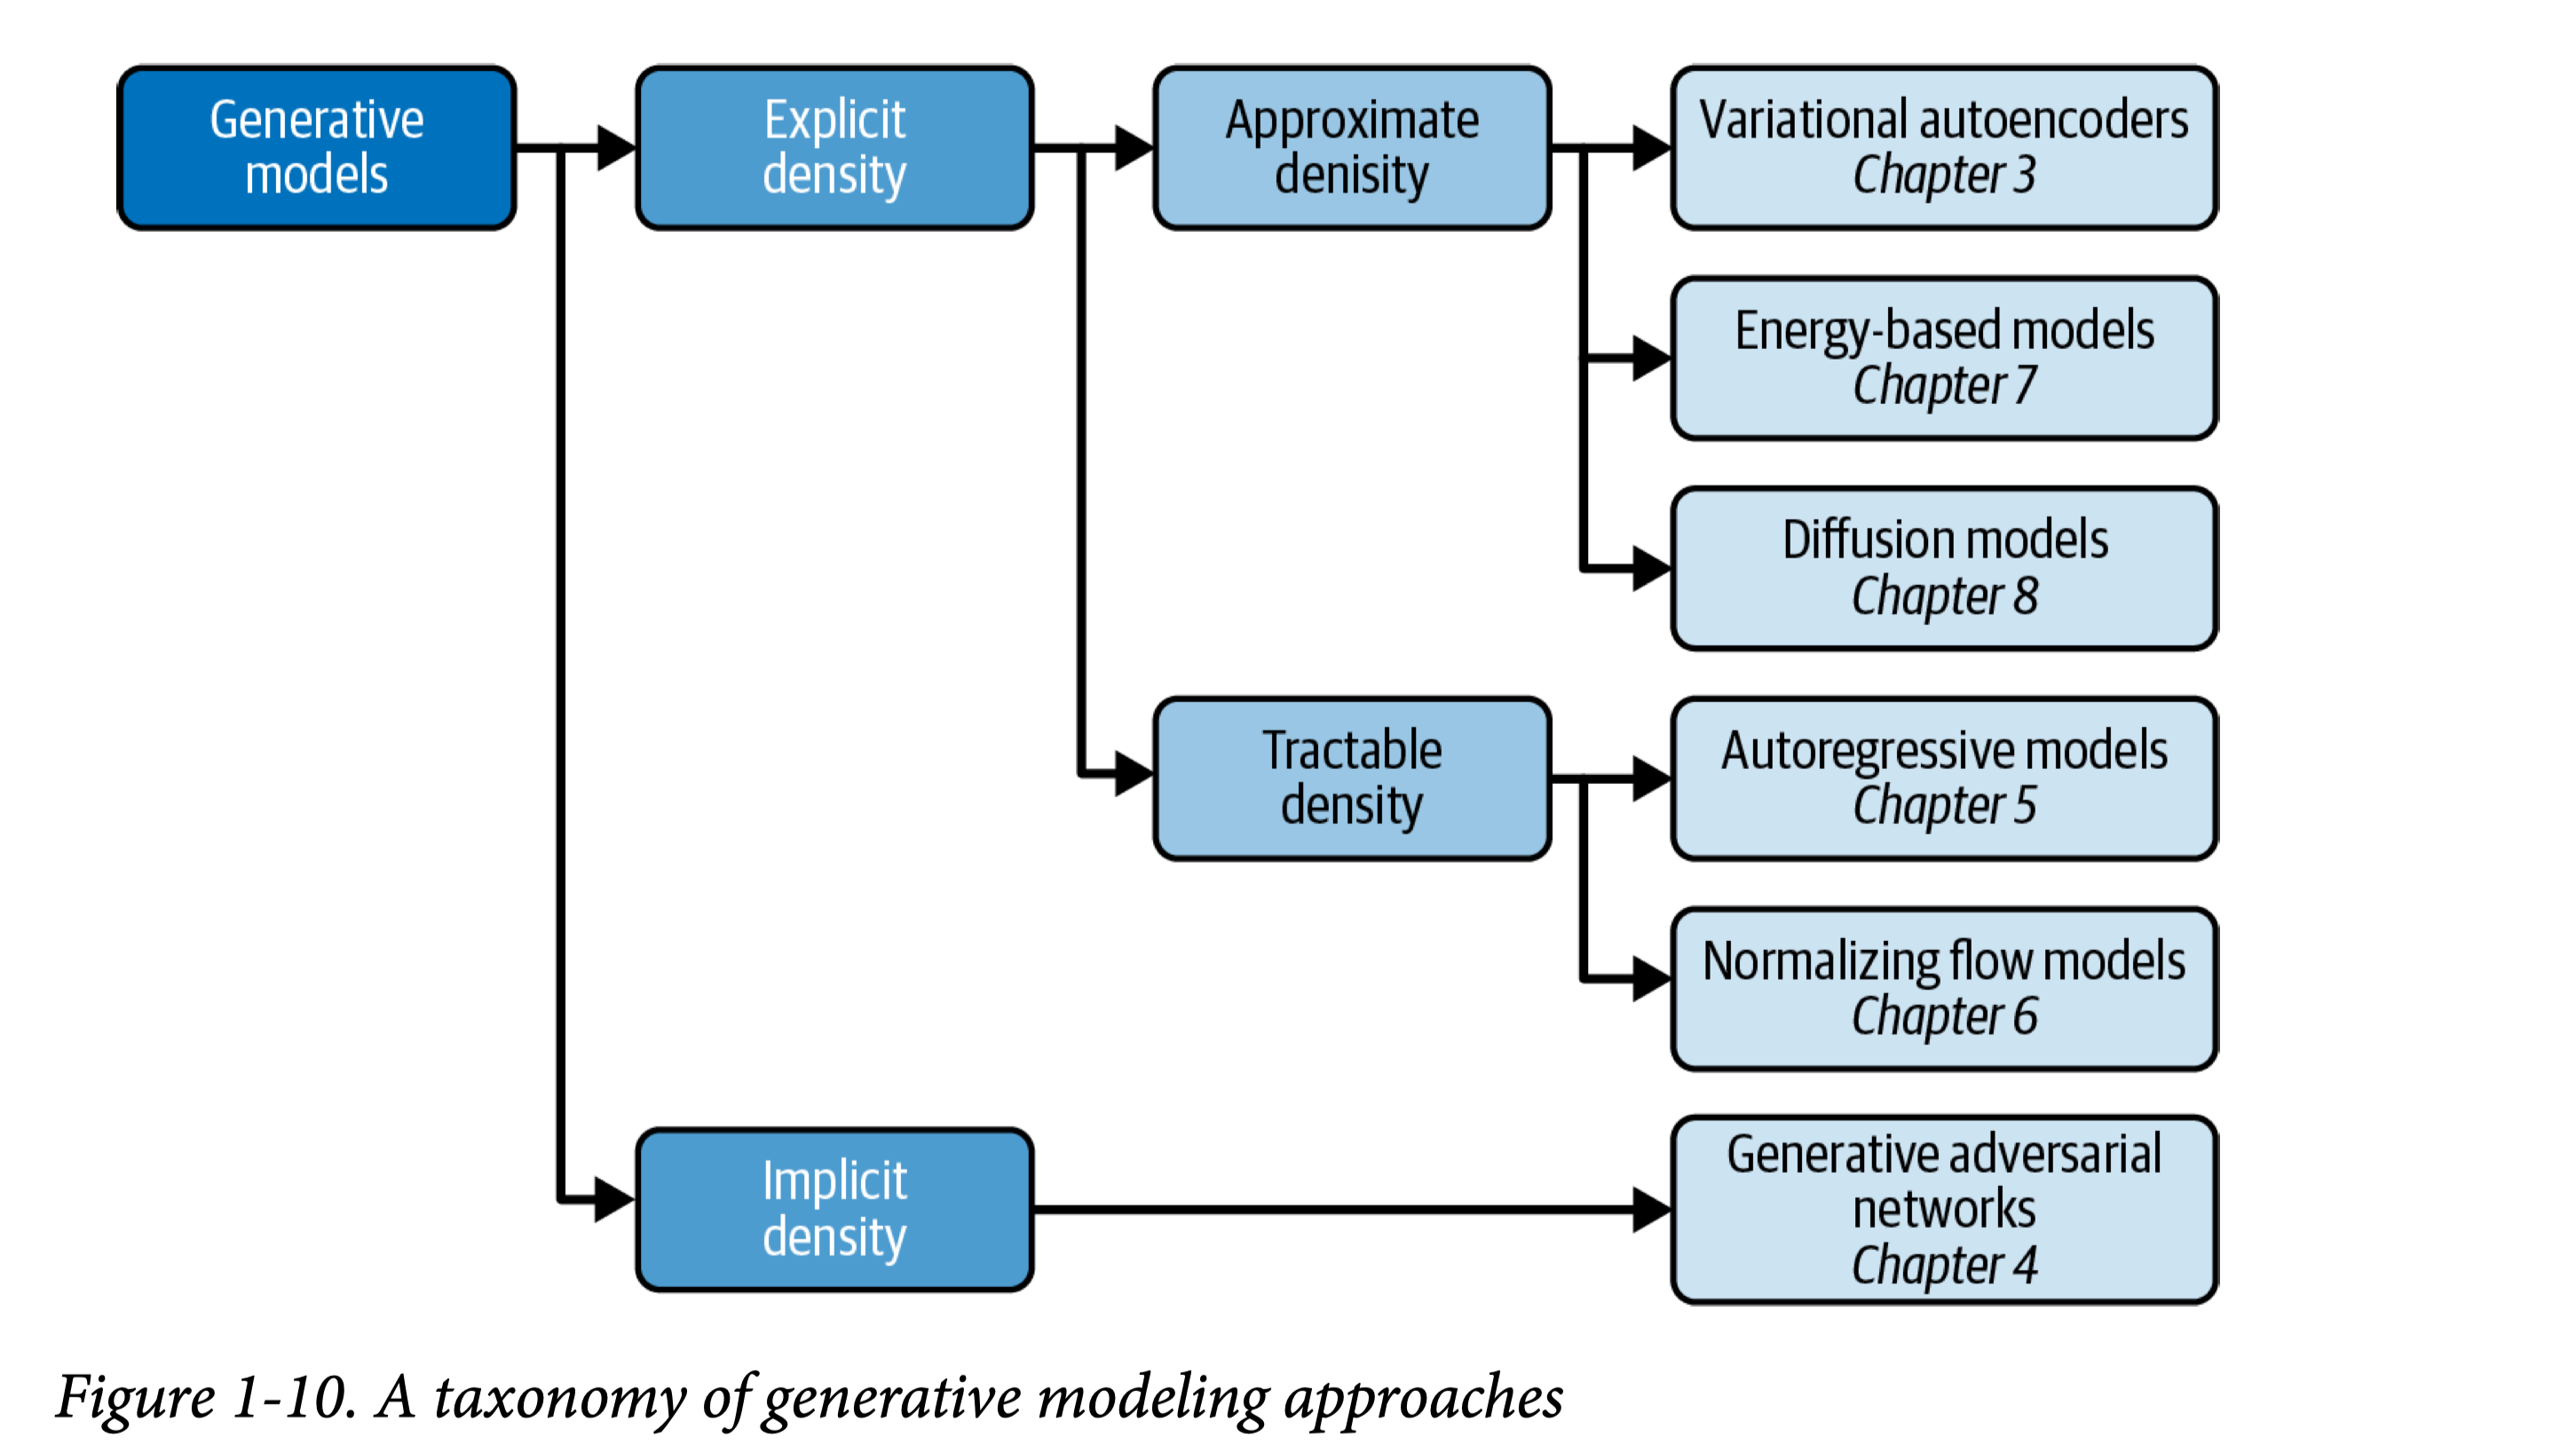
\includegraphics[width=0.95\textwidth]{figures/generative_model_taxonomy}
	\end{center}
	\caption{Generative Models Taxonomy}\label{fig:gmodel_taxonomy}
\end{figure}


If you do choose to use batch normalization before activation, you can remember the order using the acronym \textbf{BAD (batch normalization, activation, then dropout)}


\section{Variational Autoencoders}




